\documentclass{article}
\usepackage[english]{babel}
\usepackage[utf8]{inputenc}
\usepackage{graphicx}
\usepackage{hyperref}
\usepackage{booktabs}
\usepackage{multirow}
\usepackage{siunitx}
\usepackage[letterpaper,margin=0.75in]{geometry}
\usepackage[font=small,skip=-1pt]{caption}
\usepackage{amssymb}
\usepackage{amsmath}
\newcommand{\subs}{\textup{s}}
\usepackage{hyperref}
\hypersetup{
    colorlinks=true,
    linkcolor=blue,
    filecolor=blue,      
    urlcolor=blue,
    citecolor=cyan,
}

\newcommand{\subs}{\textup{s}}

\usepackage{algorithm}
\usepackage[noend]{algpseudocode}
\usepackage{etoolbox}

\makeatletter
% start with some helper code
% This is the vertical rule that is inserted
\newcommand*{\algrule}[1][\algorithmicindent]{%
  \makebox[#1][l]{%
    \hspace*{.2em}% <------------- This is where the rule starts from
    \vrule height .75\baselineskip depth .25\baselineskip
  }
}

\newcount\ALG@printindent@tempcnta
\def\ALG@printindent{%
    \ifnum \theALG@nested>0% is there anything to print
    \ifx\ALG@text\ALG@x@notext% is this an end group without any text?
    % do nothing
    \else
    \unskip
    % draw a rule for each indent level
    \ALG@printindent@tempcnta=1
    \loop
    \algrule[\csname ALG@ind@\the\ALG@printindent@tempcnta\endcsname]%
    \advance \ALG@printindent@tempcnta 1
    \ifnum \ALG@printindent@tempcnta<\numexpr\theALG@nested+1\relax
    \repeat
    \fi
    \fi
}
% the following line injects our new indent handling code in place of the default spacing
\patchcmd{\ALG@doentity}{\noindent\hskip\ALG@tlm}{\ALG@printindent}{}{\errmessage{failed to patch}}
\patchcmd{\ALG@doentity}{\item[]\nointerlineskip}{}{}{} % no spurious vertical space
% end vertical rule patch for algorithmicx
\makeatother
\usepackage{amsmath}
\DeclareMathOperator*{\argmin}{argmin}


\usepackage{listings}
\usepackage{float}
\lstset{ %
language=R,
basicstyle=\footnotesize,
numbers=left,
numberstyle=\footnotesize,
stepnumber=1,
numbersep=5pt,
showspaces=false,
showstringspaces=false,
showtabs=false,
frame=single,
tabsize=2,
captionpos=b,
breaklines=true,
breakatwhitespace=false,
escapeinside={\%*}{*)}
}

%%%%%%%%%%%%%%%%%%%%%%%%%%%%%%%%%%%%%%%%%%%%%%%%%%%%%%%%%%%%%%


\begin{document}

\title{ \normalsize 
		\\ [2.5cm] \\
		\LARGE \textbf{Area Coverage with Unmanned Aerial Vehicles\\Using Reinforcement Learning}
		\\ [0.5cm] \\}

\author{\sffamily{Research Report} \\\\ \sffamily{By} \\\\ Charles Zhang}

\date{25 May - 31 July, 2020 \\ [3.5cm] \\}

\maketitle

{
  \hypersetup{linkcolor=black}
  \tableofcontents
}
\newpage
\addcontentsline{toc}{section}{Abstract}
\begin{abstract} 

% TODO% TODO% TODO% TODO% TODO% TODO% TODO% TODO% TODO% TODO% TODO% TODO% TODO% TODO% TODO% TODO% TODO% TODO% TODO% TODO% TODO% TODO
{
\hypersetup{linkcolor=black}
\noindent In this summer research, I work with professor Esra Kadioglu-Urtis, and students Aaron Gould, Elisabeth Landgren, and Fan Zhang at Macalester College. In this project, we first implement the hexagonal tessellation area coverage approach which Esra previously published. Secondly, we develop and implement $Q$ learning reinforcement learning algorithms in a non-Markov Decision Process(NMDP) and Markov Decision Process(MDP) for the area coverage where, instead of mathematically generating a route, the drone itself will learn an efficient path to cover an entire given area and return back to its launch position. We successfully generate the shortest paths that cover a large regular or irregular field in terms of the limited drone's battery life, and finally extend the problem to include multiple drones to considerably widen the coverage area, using the Q learning and Actor Critic using Kronecker-Factored Trust Region (ACKTR) deep reinforcement learning method, built in the Gym environment in Python or by graph. My code is available at \href{https://github.com/zcczhang/UAV_Coverage}{\color{black}https://github.com/zcczhang/UAV\_Coverage}.
}
\end{abstract}

\section{Introduction}

\hspace{\parindent} The coverage path planning(CPP) for Unmanned Aerial Vehicles (a.k.a drones) are increasingly being used for many applications such as search/rescue, agriculture, package delivery, inspection, etc.\cite{1}\cite{2}\cite{3}. Using UAVs for the coverage provides several benefits, and UAVs with a high degree of mobility needs to cooperatively work as a team to provide effective coverage in a relative large are, in consideration of the limited battery life for drones\cite{4}.

Many existed work have already addressed the coverage problem by both theoretically methods or learning-based algorithms\cite{5}\cite{esra}\cite{6}. However, drones in those methods are either static for coverage in terms of drones' field of view(FOV), or only complete one-way coverage paths where the cost for the drones' recovery is not under the consideration. Therefore, in this work, we not only consider how to generate the shortest coverage paths, but also include letting the UAV return back to the launch position, which will be addressed in this work using reinforcement learning algorithms illustrated in detail in the overview sections in this report.

The main contribution of this work is to demonstrate approaches to the reinforcement learning algorithms, named Q-learning and d Actor Critic using Kronecker-Factored Trust Region (ACKTR) deep reinforcement learning, to perform the CPP of an regular or irregular environment with known obstacles, visiting only once each center of the FOV and returning(for single drone so far),  resulting in an optimized path.


% We will collect data corresponding to metrics such as the length of coverage path for a given area, maximum covered area on a single battery charge, the effect of wind and number of turns the drone makes on the battery lifetime, and analyze these results in the light of the theoretical outputs already in hand.

\section{Implementation of Hexagonal Tessellation}

\hspace{\parindent} Professor Esra Kadioglu shows that a coverage path can be obtained by using polygon tessellation of a given area, and hexagonal tessellation produces a shorter coverage path than a square tessellation, in the paper \textit{UAV Coverage Using Hexagonal Tessellation}\cite{esra}. This paper provides the algorithm to generate the Hamiltonian circuit in a rectangular field, and I implemented this algorithm to get GPS way-points given diagonal coordinates of the field and the radius of the field of view(FOV) of the UAV(\href{https://github.com/zcczhang/UAV_Coverage/tree/master/Get_Path}{code}). To improve the accuracy of the translation between longitude, latitude, and meter, I transform the coordinates to the radian first and calculate the distance showing below, with two diagonal points: (top, left), (bottom, right):
\begin{subequations}
    \begin{align}
         height = 6371000 \cdot \arccos(&\cos((top-bottom)\cdot\pi/180)),   \\
         width = 6371000 \cdot \arccos(\cos^{2}(top \cdot \pi/180) &\cdot \cos((left-right)\cdot \pi/180) + \sin^{2}(top \cdot \pi/180)), 
    \end{align}
\end{subequations}

\noindent so that: longitude per meter = (right - left) / width, and latitude per meter = (top-bottom)/height.

Figures below show two circumstances of GPS way-points for drone covering a rectangular field using hexagonal tessellation. The radius of the FOV in the left figure is 7m while 8m for the right one. 

\begin{figure}[H]
   \begin{minipage}{0.48\textwidth}
     \centering
     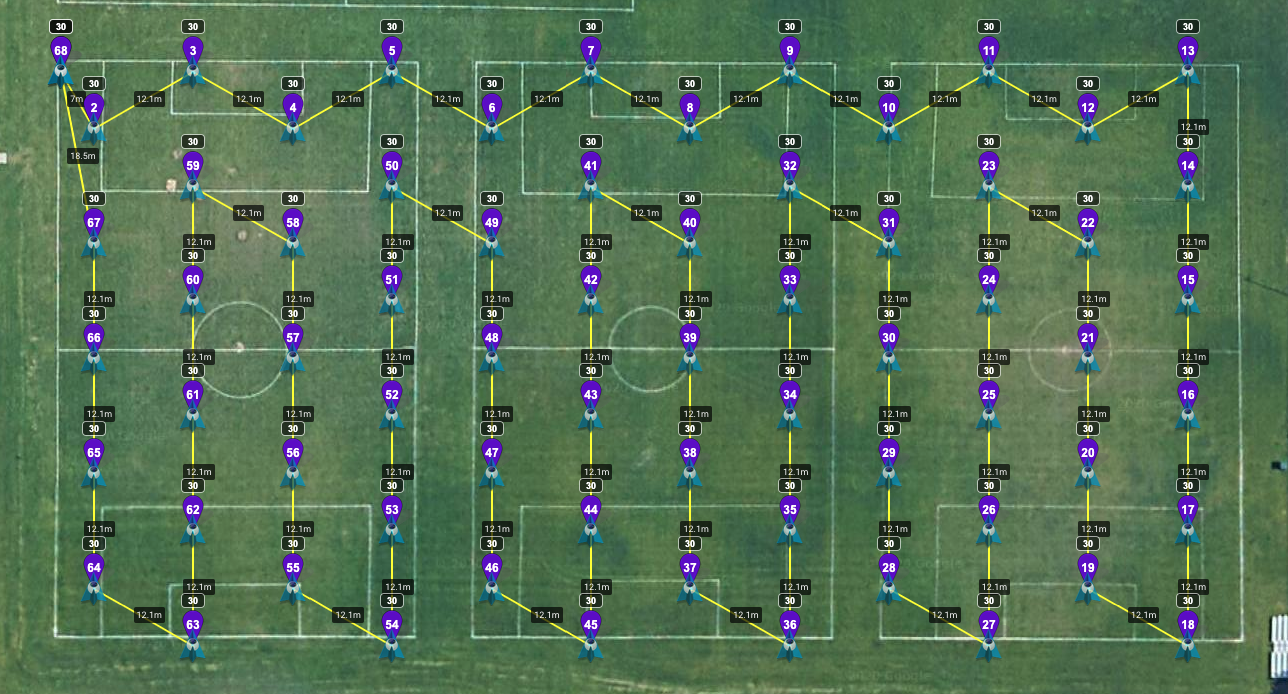
\includegraphics[width=.99\linewidth]{1.png}
   \end{minipage}\hfill
   \begin{minipage}{0.48\textwidth}
     \centering
     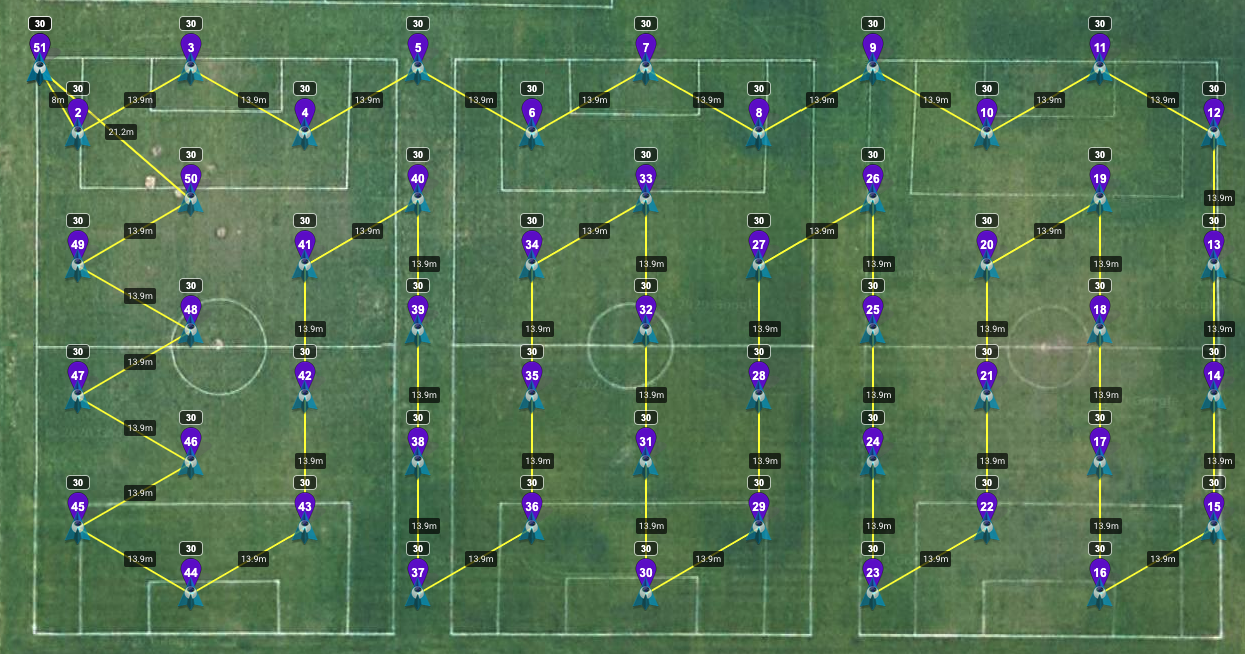
\includegraphics[width=.99\linewidth]{2.png}
   \end{minipage}
\\\caption{Two circumstances of GPS way-points for drone covering a rectangular field using hexagonal tessellation}
\end{figure}


\section{Single Agent Area Coverage}


\subsection{Overview}
\hspace{\parindent}In comparison with the hexagon tessellation which is calculated and proved mathematically that generates the shorter coverage path than the square tessellation, we want to figure out if it is possible to implement the reinforcement learning to find the shortest coverage path in a given field. To begin with, the environment is set to be the rectangular grid world, and the start point is the same with the end point. 
Specifically, the graph below gives a simple example of the rectangular 4x5 grid world where the agent starts at the (0, 0) at the upper left corner. And the drone will ideally pass through every center of the FOV, and take photos or make some other actions along with the coverage each step. Then our problem becomes to implement the reinforcement learning looking for the shortest path where the drone visits all grids(squares) and returns back to the launch position in the environment grid world.

\begin{figure}[H]
$$
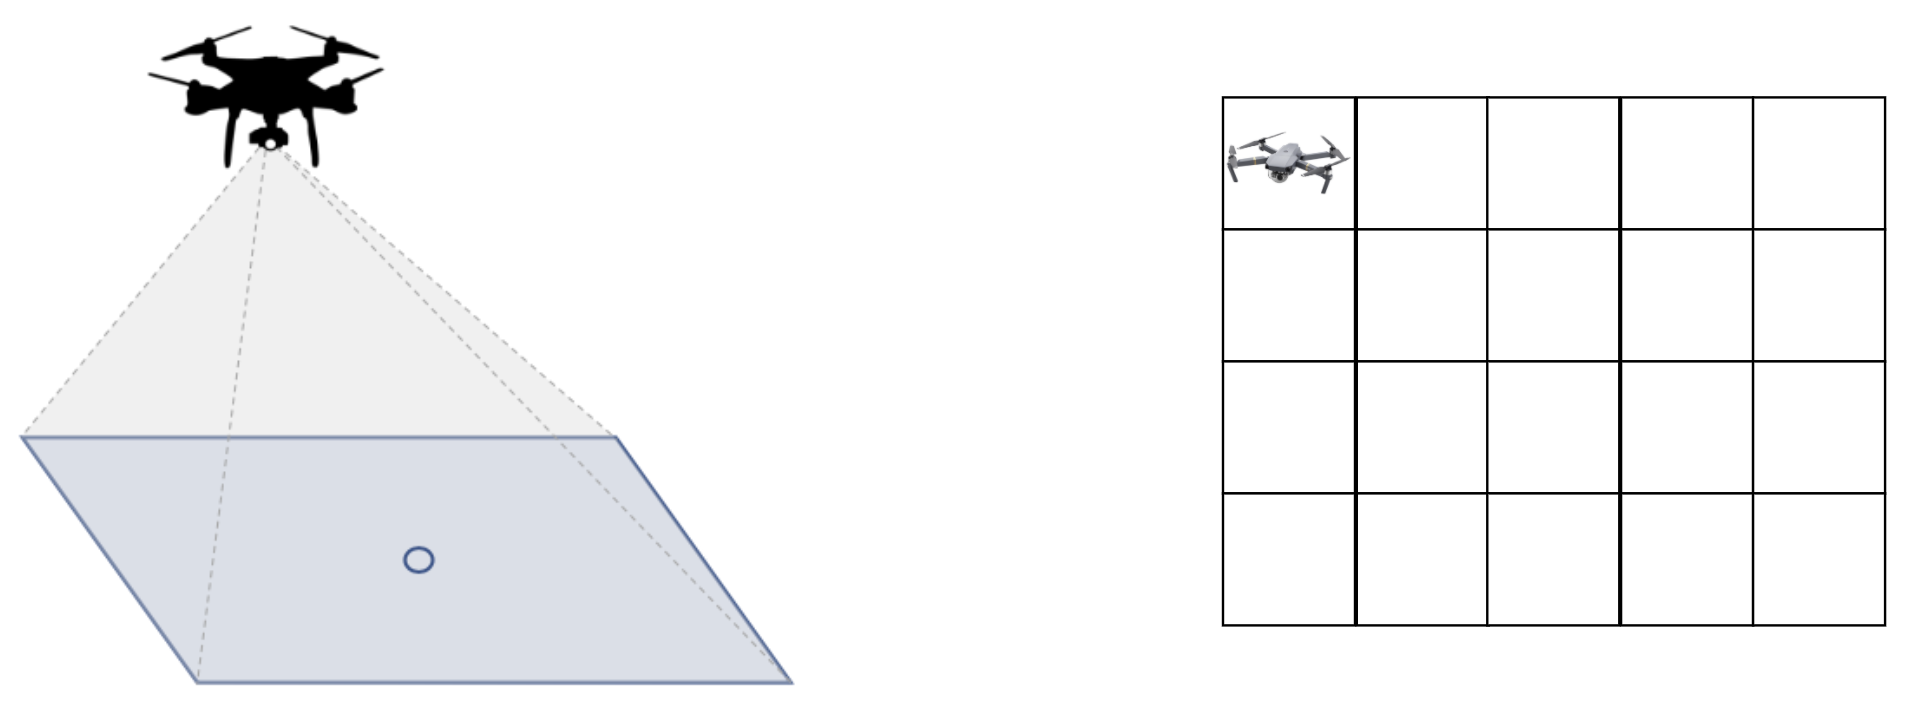
\includegraphics[width=3.5in]{3.png} 
$$
\caption{The example of a projected area of a UAV and a simple 4x5 gridworld starting at (0,0)}
\end{figure}

In this section, the whole field will be covered by one agent(a drone), using the reinforcement learning by tabular Q learning. We can define a quantity $Q(s, a)$ that equals the total reward got by executing action $a$ in state $s$. The agent will receive a huge global reward when finish the task visiting all cells and returning back to the launch position, and will receive a small penalty when revisit a cell in the gridworld, shown in the equation(\ref{eq:1}).

\begin{equation}
\label{eq:1}
R\left(S_t, A_t\right)=\left\{\begin{array}{ll}
r, & \text { if } \sum_{i} f_{i}\left(S_{t}\right) = R\cdot C \text{, and } S_t =(0,0) \\
0, & f_{i} = 0 \\
-1, & \text { otherwise }
\end{array}\right.
\end{equation}
where $r$ is a relatively large constant reward and $f_i:\{S\} \rightarrow \{0,1\}$ shows whether the state is visited, where 0 for unvisited while 1 for visited. The value function can be defined via the value $V(s)$ as an expected total reward (optionally discounted) that is obtainable from the state. 
This quantity gave a name to the whole family of methods called Q-learning\cite{drl}. Applying the bellman equation and temporal difference method, the tabular Q learning updates the Q value $Q(S,A)$ corresponding with the state $s$ and action $a$ after each step, showing following:

\begin{equation}
\label{eq:q}
   Q(S, A) = (1-\alpha) \cdot Q(S, A) + \alpha \cdot (R + \gamma \cdot \max_{a} Q(S’, a))
\end{equation}
where $S$ and $S'$ are the current and next (potential) states respectively; $R$ is the reward based on the current state $s$ and action $a$; $\alpha$ is the learning rate; and $\gamma$ is the discount factor\cite{drl}. In our research, the state is set to be the waypoint of the environment---the gridworld in this section.  


\subsection{NMDP Tabular Q Learning}
\hspace{\parindent} Since in each step in each episode, the agent has to observe if the current state is visited or not in order to get the reward, instead of only observing the current state, the process is the non-Markov Decision Process(NMDP). In order to let the agent "learn" faster, I assume that they will visit the unvisited grid first. I also implement the decaying epsilon-greedy method to maximize the numerical reward for the action policy $\pi(s)$ for each state $s$, shown below,

\begin{equation}
\label{eq:2}
    \pi(s)=\left\{\begin{array}{ll} a \in A, & \mathbb{P} = \epsilon \\ a \in \arg \max _{a\prime} Q_{k}\left(s_{k}, a\prime\right), & \mathbb{P} = 1-\epsilon \end{array}\right.
\end{equation}
where $\epsilon$ decreases over time proportionally. Since the agent has to finish two task for each episode: visit all grids and complete the loop back to the origin, the agent will randomly move and receive the reward when visit the unvisited grid, and will receive a much larger global reward for both finishing visit and coming back. Instead of terminating the episode once the agent re-visit a state where leads to a "fail" for the shortest coverage task like most reinforcement learning algorithms, my algorithm allows the repetition of visits but the agent will receive a negative reward for the penalty, in order to make the agent "learn" and distinguish faster both from the good decisions and bad decisions\cite{rl_sutton}. The algorithm below shows the tabular Q learning for one agent looking for the optimal path.
\begin{figure}[H]
  \centering
  \begin{minipage}{.7\linewidth}
  
\begin{algorithm}[H]
\caption{NMDP Tabular Q Learning for Area Coverage} 

\begin{algorithmic}[1]
\State Initialize the environment $R\times C$ board
\State Initialize state space $\mathcal{S} = \{(0,0), \dots, (ROWS-1, COLS-1)\}$
\State Initialize action space $\mathcal{A} = \{'\text{up}', '\text{down}', '\text{left}', '\text{right}'\}$, prefer to visit unvisited grid first
\State Reward function $R: \mathcal{S} \times \mathcal{A} \rightarrow \mathcal{R}$
\State Initialize Q table $Q: \mathcal{S} \times \mathcal{A} \rightarrow \mathcal{R}$ arbitrarily 

\While{not reach the number of episodes} 
    \State $S  \gets$ random $S \in \mathcal{S}$
    \While{not reach END \textbf{and} not visit all}
        \State set $S$ as visited
        \State choose $A \in \mathcal{A}$ using policy $\pi(S)$ [\ref{eq:2}]
        \State take $A$, observe $S'$ whether it is visited, and get $\mathcal{R}$
        \State $Q(S, A) \gets (1-\alpha) \cdot Q(S, A) + \alpha \cdot (R + \gamma \cdot \max_{a} Q(S’, a))$
        \State $S \gets S’$
        \State decay $\epsilon$ proportionally
        \EndWhile
        
\State \textbf{end}
    \EndWhile
    
\State \textbf{end}
        
\end{algorithmic}
\end{algorithm}

  \end{minipage}
\end{figure}

\noindent where $S$ and $S'$ are the current and next states respectively; $\mathcal{R}$ is the reward based on the action $a$ referring to $S$, which is dependant on whether the agent visit unvisited states, and finish the coverage task as well as flying back; $\alpha$ is the learning rate; and $\gamma$ is the discount factor. 

During the training, 4 values corresponding with four available directions up, down, right, and left at each entry of the $ROWS\times COLS$ table of $Q$ values will be updated. The policy for the greedy method will choose the direction with the largest value at each state in the gridworld. After training, optimal path could be derived by choosing the direction with the largest $Q$ value among all directions each state from the $Q$ table. Since the movements at the beginning are random, and there are more than one "optimal paths" which go through all grids exactly once and get back to the origin, we could get different Q tables and paths after training(\href{https://github.com/zcczhang/UAV_Coverage/blob/master/Grid\%20World/Past_All_Grids_v2.0.1.ipynb}{code}). Then, two different results of coverage path in a simple 4$\times$5 gridworld are illustrated in figure 3 and figure 4. The table of directions corresponding with the largest $Q$ values in the $Q$ table is shown at the left, while the derived coverage path is shown at the right by dotted arrows. In conclusion, the minimum steps which is equivalent to the shortest coverage distance is supposed to be 20 steps in $4\times5$ gridworld, which is consistent with results derived by this reinforcement learning algorithm shown below. 

\begin{figure}[H]
$$
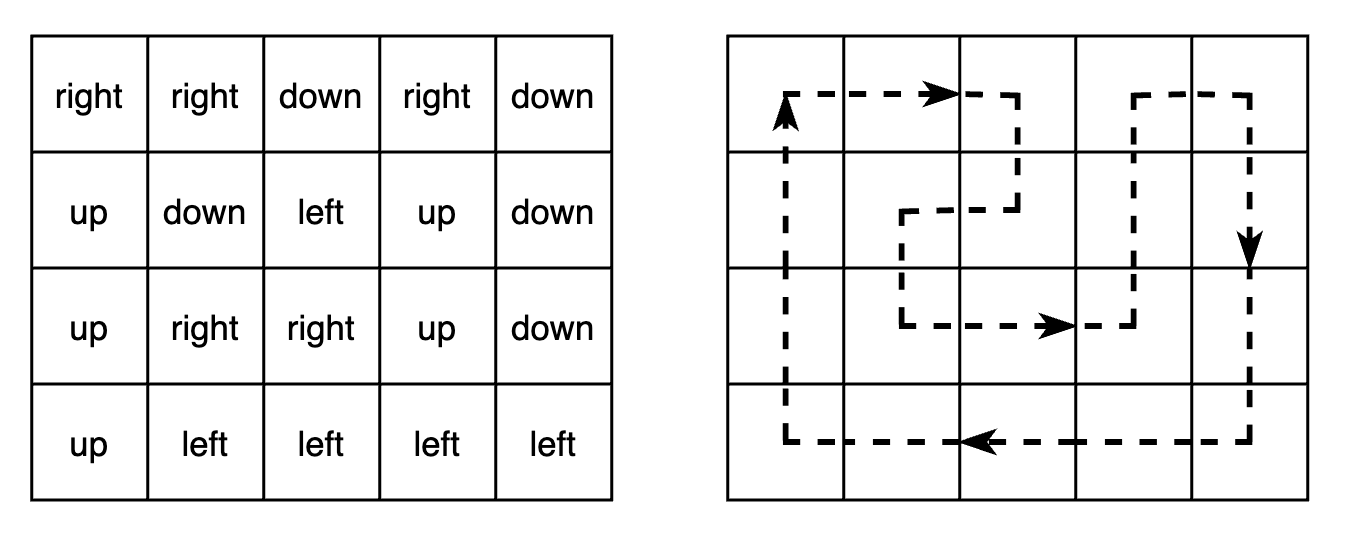
\includegraphics[width=4in]{5.png} 
$$
\caption{The first coverage path generated by NMDP tabular Q learning in 4x5 gridworld}
\end{figure}

\begin{figure}[H]
$$
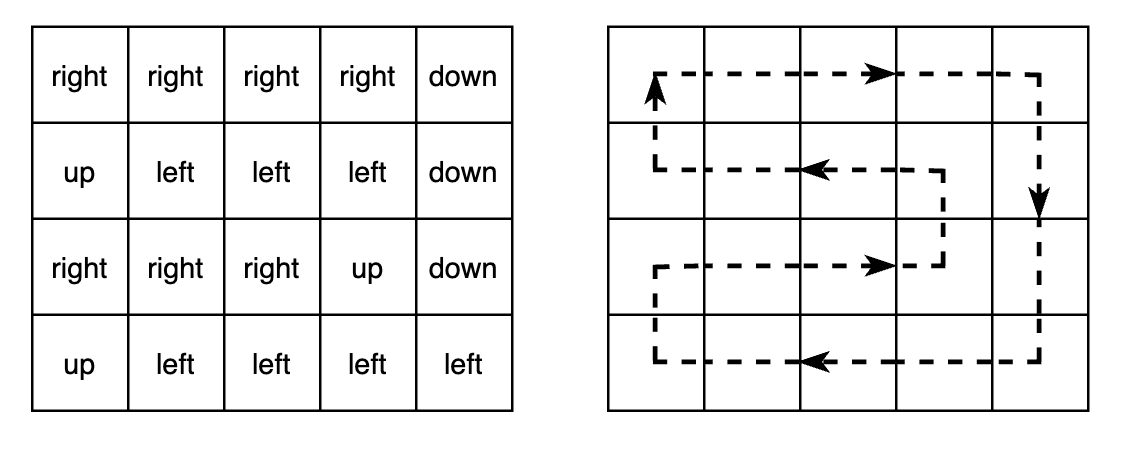
\includegraphics[width=4in]{7.png} 
$$
\caption{The second coverage path generated by NMDP tabular Q learning in 4x5 gridworld}
\end{figure}

The convergence means that the policy for shortest coverage path planning from $Q$ values will not be changed, and the steps equal to the shortest distance for visiting all states and return back, which is the number of grids in the gridworld. From figure 5 and figure 6 represented the number of steps each episode, steps will converge around 350 episodes in the $4\times5$ gridworld. Using the decaying epsilon-greedy method can make sure that the agent will converge to only one optimal path for each training, and this is also the reason why multiple different results would be generated for each training. The steps vibrate a lot at the beginning and after the convergence, since a random state in the environment will be chosen to be the start state each episode. This random start state will make sure the agent looking for an optimal direction at any state for visiting all cells and getting back. The number of steps is increasing at first because the agent is sticking to a path that cover some but not all grids and the agent has less and less probabilities due to the decaying $\epsilon$-greedy policy to be broken away from the current local optimum, but the number of cells for these repeatedly visited loops is actually increasing while training. And once the visited grids for the loop that the agent is sticking on each episode equal to the number of all grids in the grid world, the step will converge “suddenly” to the optimal steps, the number of grids in the gridworld, showing as the steep decrease just before the convergence around 200 to 300 episodes in this case. 

\begin{figure}[H]
   \begin{minipage}{0.48\textwidth}
     \centering
     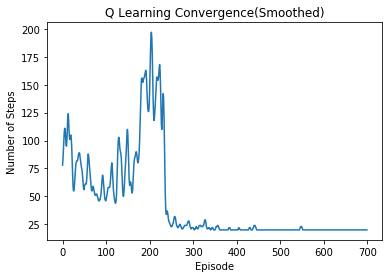
\includegraphics[width=.99\linewidth]{4.png}
     \caption{The first convergence for tabular Q learning in 4x5 gridworld}\label{Fig:Data1}
   \end{minipage}\hfill
   \begin{minipage}{0.48\textwidth}
     \centering
     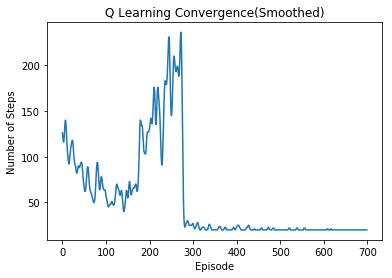
\includegraphics[width=.99\linewidth]{6.png}
     \caption{The second convergence for tabular Q learning in 4x5 gridworld}\label{Fig:Data2}
   \end{minipage}
\end{figure}

This naive tabular Q learning could also be implemented in the hexagon tessellation environment by allowing six directions up, upper left, upper right, down, bottom left, and bottom right. Then, it requires a larger dimension of action space and $Q$ table, and many out-of-bound directions need to be considered. Besides, as the size of the gridworld becomes large, it is unstable to find the coverage solution. Therefore, in the next section, a graph based algorithm will be introduced to reduce the computation and be available for more complicated environment like irregular field with obstacles.


\subsection{Graph Based MDP Q Learning}

\hspace{\parindent} In this section, I set the environment as a graph, where the vertices are the state that need to be covered and edges are available directions that the agent drone can fly through. Then, using adjacency matrices, only attainable vertices will have corresponding values for $Q$ values, rewards, and actions. In this way, more complicated real world environment beyond the gridworld can be transformed to the graph to implement reinforcement learning\cite{GBQL}. Assume the environment has $V$ vertices, then $R$ and $Q$ are $V\times V$ matrices. Specifically, $R$ is an adjacency matrix except $R[i,j]$ where $j$ is the end(start) state and $i, j$ are connected. In this way, each step of exploration will get a small reward except reaching the end state with a much larger reward. Unlike the NMDP naive Q learning in the previous section, the agent will first find shortest paths from any state in the environment to the launch position, and then store the $Q$ values in $Q$ matrix. This process is MDP, and is straightforward to implement the $Q$ learning. As actions for the agent in this MDP are fully random without greedy move, the simple bellman equation is better to use to update Q values recursively\cite{drl_5}.

\begin{equation}
    Q(S,a) = R(S,a) + \alpha \cdot \max_a Q(S’, a’)
\end{equation}

To get the solution for coverage path planning, I consider that if the agent is supposed to to cover all grids, or in other words visit more states, it is equivalent to avoid the shortest path and minimize the overlapping states, by choosing the minimum Q value for the policy. The algorithm of this $Q$ learning with graph-based state representation is shown below,

\begin{figure}[H]
  \centering
  \begin{minipage}{.7\linewidth}
  
\begin{algorithm}[H]
\caption{Graph-Based State Q Learning for Area Coverage} 

\begin{algorithmic}[1]
    \State Initialize state space $\mathcal{S} = \{1, \dots, V\}$
    \State Initialize action space and reward matrix $\mathcal{R}$: $R[S, a]$, $\forall S, a$
    \State Initialize Q table $\mathcal{Q}$: $Q[S, a] =  null$,  $\forall S, a$ 
    \While{not reach the number of episodes} 
        \State $S  \gets$ random $S \in \mathcal{S}$
        \While{$S \neq END$}
        \State $a \gets$ random $a$ valid in the $S$
		\State $S’ \gets a$
		\State $Q[S, a] \gets R[S,a] + \alpha \cdot \max_a Q[S’, a’]$
		\State $S \gets S’$
        \EndWhile
        
\State \textbf{end}
    \EndWhile
    
\State \textbf{end}

\State $S = START$   
\State $Path$ is an empty list for the shortest path
\While{length($Path$) $< V$}
    \State add $S$ to $Path$
	\State $S’ \gets S$
	\State $S \gets \argmin (Q[S, \text{ }])$
	\State $Q[S’,\text{  }] \gets null$
	\State $Q[\text{     }, S’] \gets null$
\EndWhile
\State \textbf{end}
\end{algorithmic}
\end{algorithm}

  \end{minipage}
\end{figure}

\noindent where $R[S,a]$ is the reward based on the action $a$ referring to $S$. As this algorithm only considers the accessible directions for connected vertices reflected by 1 in the adjacency matrix, and only $Q[i,j]$s with connected $i,j$ are updated, the computation for updating $Q$ values reduces significantly so that more accurate solutions in larger environment can be realized. For example, $20\times 20$ gridworld is transformed as the graph where the indices of vertices are from 1 to 400, shown at the left of figure 7, and the optimal coverage path is generated by this algorithm after training only 500 episodes is visualized at the right(\href{https://github.com/zcczhang/UAV_Coverage/tree/master/Graph_Based_Coverage}{code}).

\begin{figure}[H]
     \centering
     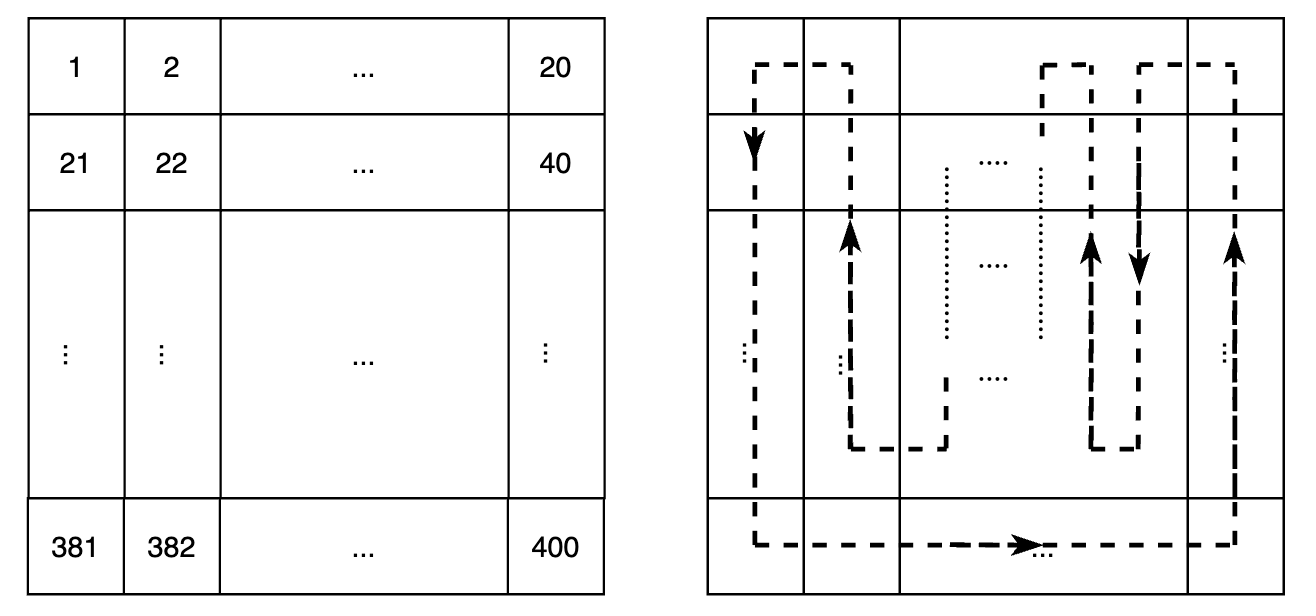
\includegraphics[width=3.5in]{8.png}
     \caption{20x20 graph of gridworld and the solution for its coverage path planning}
\end{figure}

The pattern of the output path for the other sizes of gridworld generated by algorithm 2 are all supposed to be the zigzag path, similar with $20\times20$ gridworld visualized above. It is perspicuous to prove that this is the shortest coverage path as well as Hamiltonian cycle for the squared tessellation in the gridworld: the shortest coverage path is the number of vertices times the distance between two centers of two adjacent squares, which is consistent with the zigzag coverage path generated by Q Learning with Graph-Based State Representations.

In comparison with \textit{Algorithm 1}, this algorithm is much more efficient to be implemented in the hexagonal tessellation or irregular field environment, since the action space is simplified to only include actions for reachable adjacent directions and the update of action and Q table are similar with the computation of adjacent matrices. Then, this algorithm is tested in the hexagonal tessellation of rectangular environment and two produced solutions of coverage path are shown in figure 8. The algorithm successfully produces the optimal coverage path, where the solution at the left has the same path with what Esra mathematically generated and proved to be the shortest Hamiltonian circuit coverage path\cite{esra}. It is relevant to be considered in the future work that though two solutions have the same total distances for both UAV coverage and returning to the launch location, the second solution has more turns affecting the time of completion and battery use, which is not considered during the learning in the algorithm so far.  

\begin{figure}[H]
     \centering
     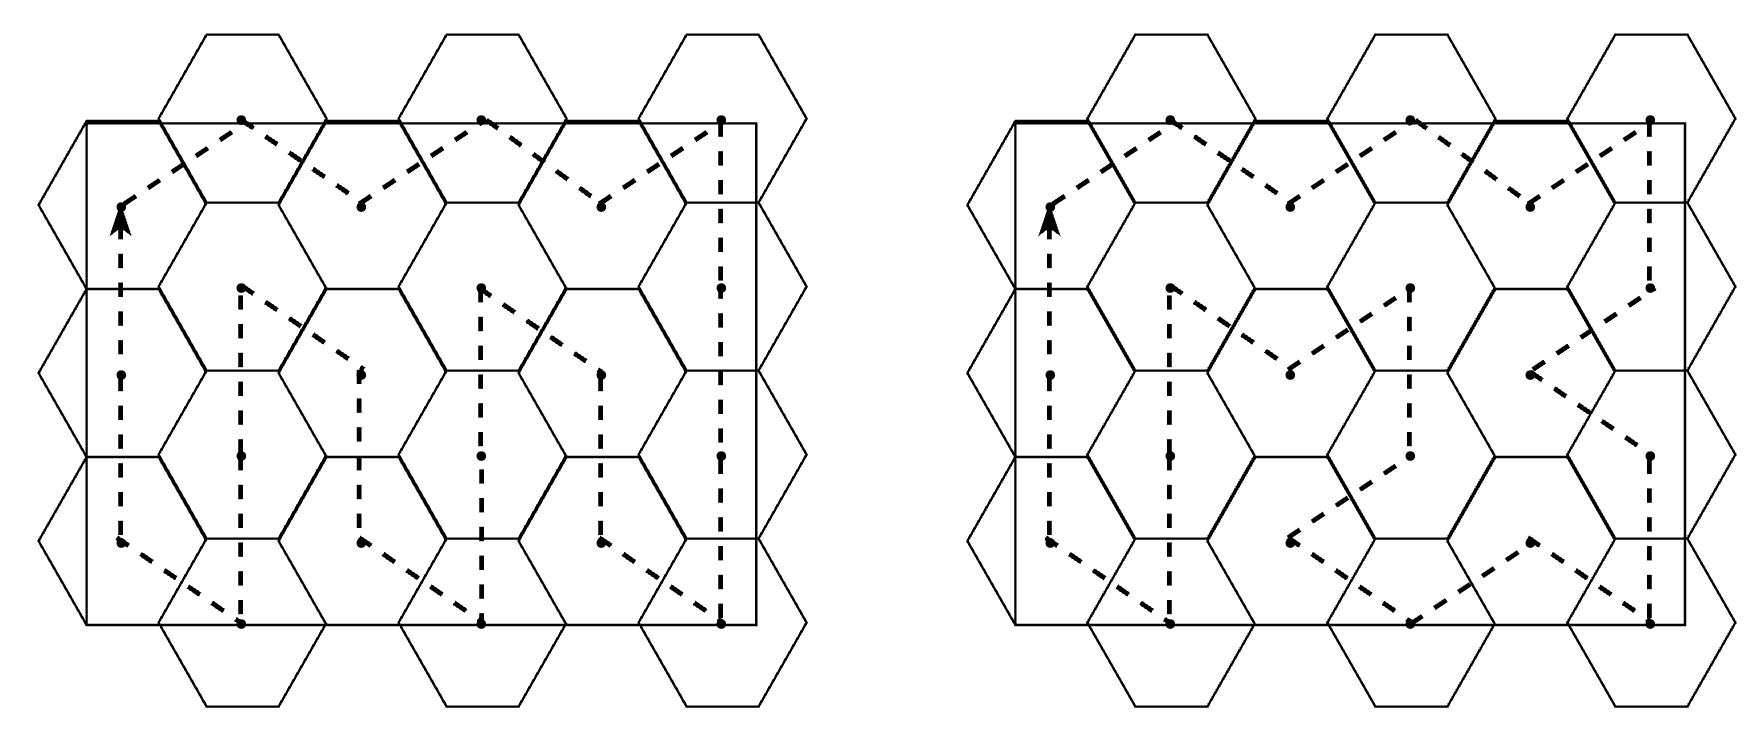
\includegraphics[width=4in]{11.png}
     \caption{Two solutions of coverage path in hexagonal tessellation of rectangle environment}
\end{figure}

In figure 9, the irregular field environment is tested. The light blue area at the left is the area that the drone need to cover, and shadow blocks are obstacles that the drone does not need to cover. Then the square tessellation where the center of each FOV of the drone is the position that the drone will pass and take photos or make actions along with the coverage, and the optimal Hamiltonian circuit path is shown at the right.

\begin{figure}[H]
     \centering
     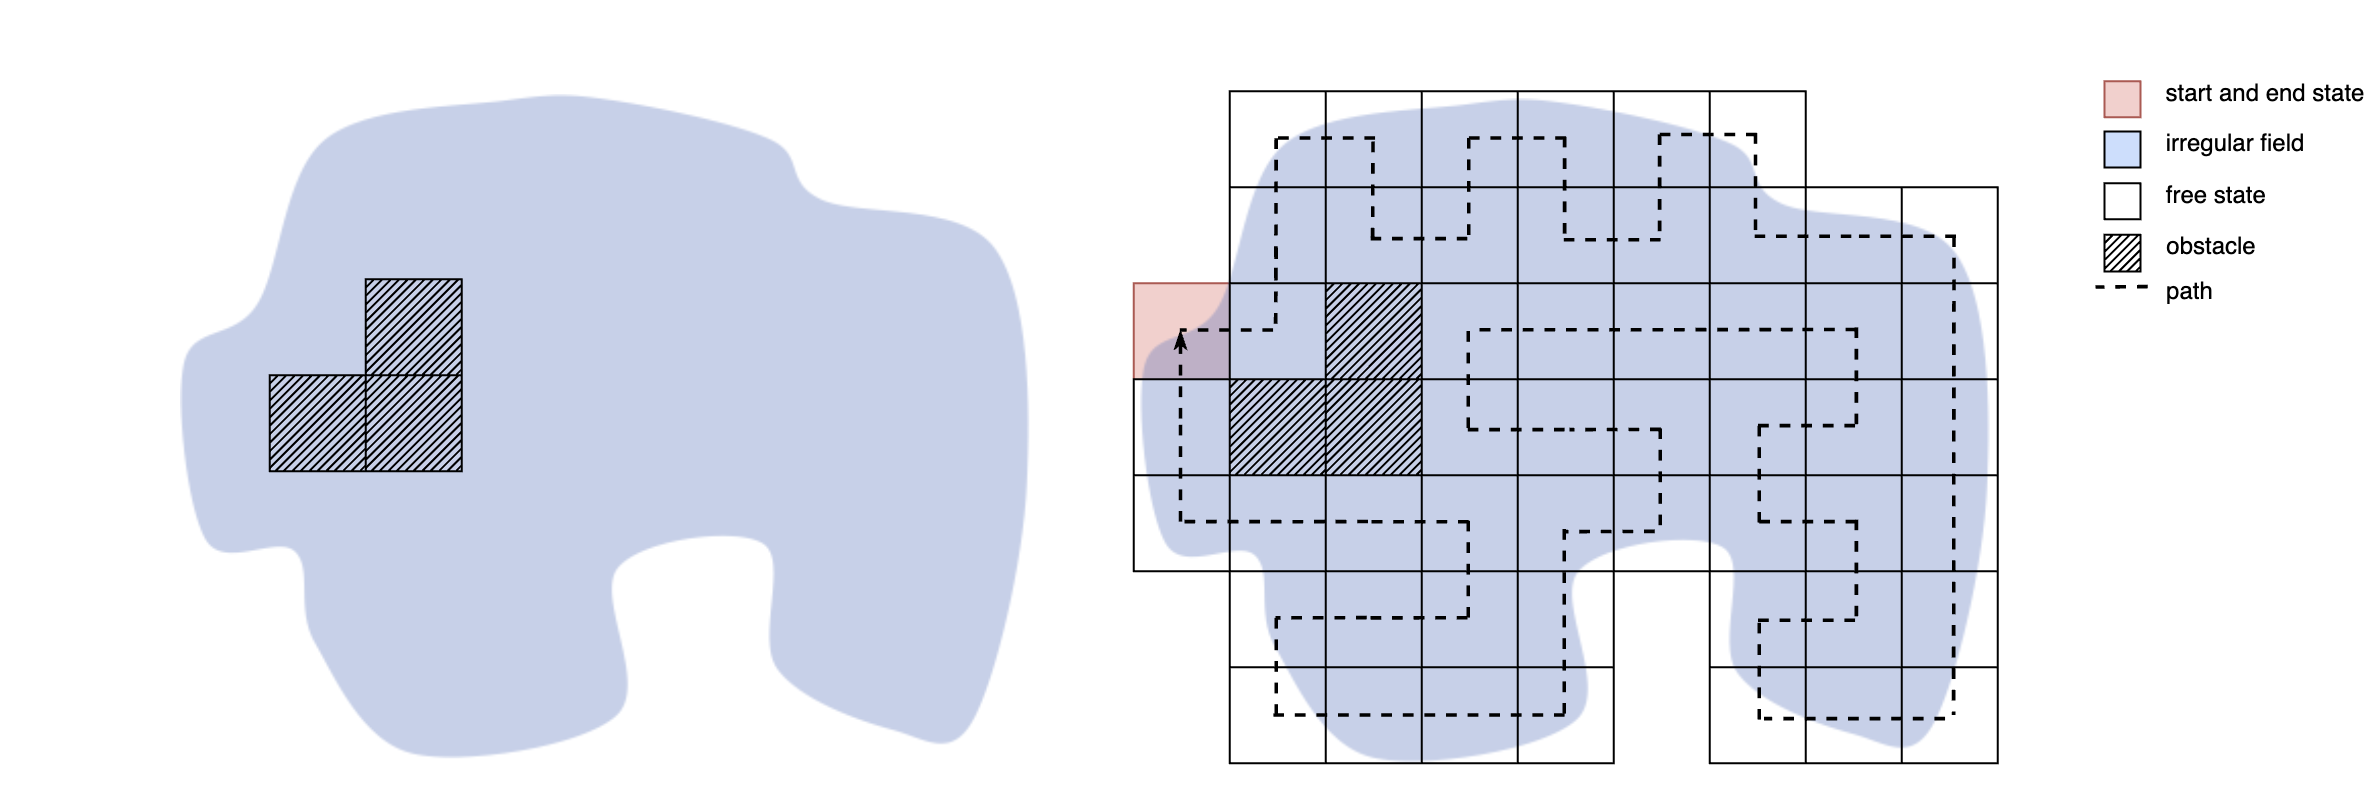
\includegraphics[width=.9\textwidth]{10.png}
     \caption{Solution of coverage path in an irregular field environment}
\end{figure}

Therefore, our graph-based state Q learning for area coverage could provide the coverage for a larger size of a regular or irregular field for a single UAV than the algorithm in the Section 3.2. However, this algorithm is not to directly find the optimal shortest distance for the area coverage, we could not observe whether the agent will successfully find the solution straightforward during or after the training, and this algorithm will be hard to extend to the multi-agents coverage. 

\newpage

\section{Dual Agents Area Coverage}

\subsection{Overview}
\hspace{\parindent} Normally, the battery for the single UAV could not guarantee the area coverage in a large field, so we try to find out solutions for multi-drones cooperatively providing the coverage by reinforcement learning. In this research, we focus more on the double agent area coverage. Similar with the environment for the single agent, we first build our environment in the gridworld, while the first agent will be launched at the $0,0$ at the upper left corner in the board, and another agent will be launched at $(ROWS-1, COLS-1)$ at the bottom right corner in the board, illustrating in figure 10.

\begin{figure}[H]
     \centering
     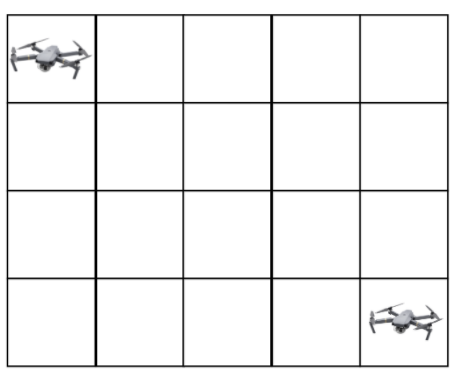
\includegraphics[width=.25\textwidth]{19.png}
     \caption{The example of simple 4x5 gridworld starting at (0,0) and (3,4) for two drones}
\end{figure}

In comparison with the environment for the single agent, we consider two coordinates as well as two actions for each state and action space, which will be updated each step simultaneously for two drones. Then, the $Q$ table can be considered two separate $Q$ table for each drone with 4 directions in each coordinate, but also can be considered as one $Q$ table which include action space with $4\times 4$ directions and state space of all combinations of possible coordinates in the board. In consideration of the exponentially increased computation of the reinforcement learning for double even multi-agents coverage, we abandon the task for returning back to the launch back, so that both agents are supposed to stop once they cover all grids in the gridworld(the distance then go back to the launch position is not under the consideration in this case). Then, in each state, the reward and next action will be only dependent on whether current grids are visited or not, so this process would be considered as the Markov decision process(MDP) $(S, A, \gamma, P, r)$. At time $t$ and state $s_t\in S$ of two coordinates in the gridworld, the two drones which will be integratedly observed as one agent chooses an action $a_t$ of two directions according to the policy $\pi(a_t|s_t)$ same with Eq.\ref{eq:2} of single drone area coverage. After receiving the action, the environment produces a reward $r_{t+1}$ and
transitions to the next state $s_{t+1}$ according to the transition probability $P(s_{t+1}|s_t,a_t)$. The process continues until the agent reaches a terminal state. The goal of the agent is to maximize the expected discounted cumulative rewards under the policy $\pi$ with discount factor $\gamma\in (0, 1]$. In this section, we update the reward function similar with how to feed reward for the single agent as Eq.\ref{eq:1}, by:
\begin{equation}
\label{eq:mrl_r}
R\left(S_t, A_t\right)=\left\{\begin{array}{ll}
r, & \text { if } \sum_{i} f_{i}\left(S_{t}\right)+\sum_{i}g_{i}\left(S_{t}\right) = R\cdot C \\
0, & f_{i} = 0 \text{ or } g_{i} = 0\\
-1, & \text { otherwise }
\end{array}\right.
\end{equation}
where $f_i, g_i:\{S\} \rightarrow \{0,1\}$ shows whether two grids for each state are visited by drones $f$ and $g$, where 0 for unvisited while 1 for visited; and $r = 2\cdot R\cdot C - \left(|i_0-i_0'|+|j_0-j_0'|+|i_1-i_1'|+|j_1-j_1'|\right)$ for states $s_t=((i_0,j_0),(i_1,j_1))$ and $s_{t+1}=((i_0',j_0'),(i_1',j_1'))$ after $a_t$. Then, we still train our model by using the tabular $Q$ learning applying the bellman equation and temporal difference method to update $Q(S,A)$ corresponding with the state $s$ and action $a$ after each step with the Eq.\ref{eq:q}.


\subsection{Multi-Agents Q Learning}

\hspace{\parindent} If we do not consider the complex dimension of the state space, action space, and $Q$ table, our method could be generalized as the tabular Q learning for $n$ drones area coverage, where we could use $n=2$ for our double drones area coverage. Since all exactly same drones will take actions simultaneously, we consider this multiple drones system as one agent, and then implement the tabular $Q$ learning similar with the single agent tabular $Q$ learning and with same denotations, shown below\cite{mul_q}. 

\begin{figure}[H]
  \centering
  \begin{minipage}{.7\linewidth}
  
    \begin{algorithm}[H]
    \caption{Multi-Drones tabular Q Learning for Area Coverage} 
    
        \begin{algorithmic}[1]
        \State Initialize the environment $R\times C$ board and $n$ agents
        \State Initialize $\mathcal{S}=(s_0,s_1,...,s_n), s_i \in \{(0,0),\dots, (R-1, C-1)\}, 0\leq i \leq n$
        \State Initialize $\mathcal{A} = (a_0,a_1,...,a_n), a_i\in\{'\text{up}', '\text{down}', '\text{left}', '\text{right}'\}, 0\leq i \leq n$
        \State Reward function $R: \mathcal{S} \times \mathcal{A} \rightarrow \mathcal{R}$
        \State Initialize Q table $Q: \mathcal{S} \times \mathcal{A} \rightarrow \mathcal{R}$ arbitrarily 
        
        \While{not reach the number of episodes} 
            \State reset $S=(s_0, s_1,...,s_n)$ to their initial positions
            \While{not cover all in board}
                \State set $s_0, s_1,...,s_n$ in $S$ as visited in board 
                \State choose $A=(a_0, a_1,...,a_n)$ using policy [\ref{eq:2}] for each $a_i$, $0\leq i \leq n$
                \State $S' = (s_0', s_1',...,s_n')$
                \State observe $s_i'$, $0\leq i \leq n$ whether it is visited, and get $
                \mathcal{R}$
                \State $Q(S, A) \gets (1-\alpha) \cdot Q(S, A) + \alpha \cdot (R + \gamma \cdot \max_{a} Q(S’, a))$
                \State $S \gets S’$
            \EndWhile
                
        \State \textbf{end}
            \EndWhile
    
        \State \textbf{end}
                
        \end{algorithmic}
    \end{algorithm}

  \end{minipage}
\end{figure}

We then conduct our experiment for the dual drones coverage in the $5\times6$ gridworld by initializing $n=2$ in the algorithm(\href{https://github.com/zcczhang/UAV_Coverage/tree/master/multi_agent_Q_Learning}{code}). Figure 11 and figure 12 shows two successful convergences of steps each episode for this algorithm in the $5\times6$ gridworld. In this case, each step is moving from a center of a grid to another center of a grid, and the convergence means that the agent of two drones finish providing the coverage in a stable steps for all 30 grids and the $Q$ table will not be updated. From figures below, we could see that the agent could find a relatively small steps after training and our agents are indeed learning.

\begin{figure}[H]
   \begin{minipage}{0.49\textwidth}
     \centering
     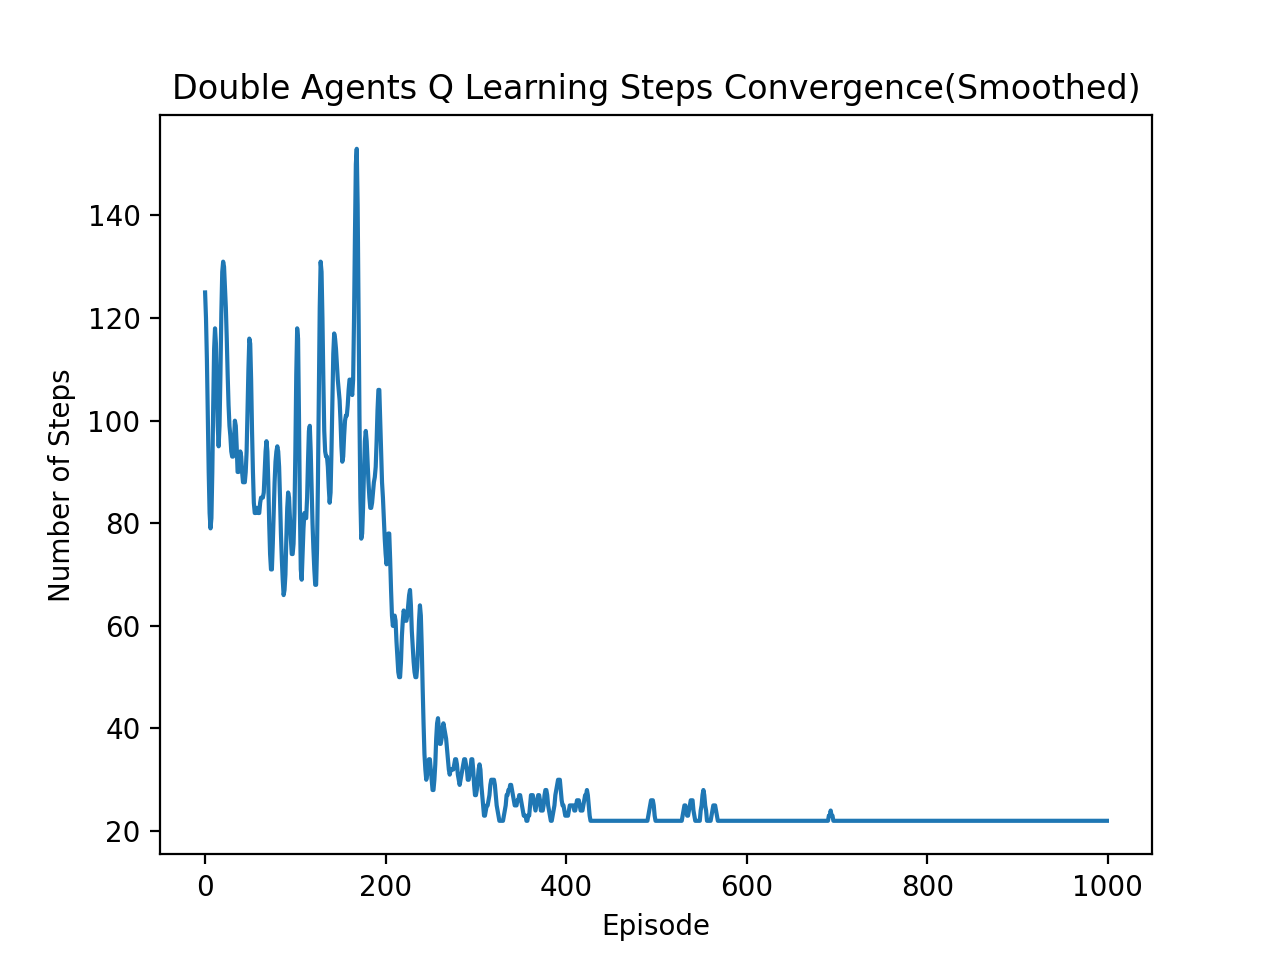
\includegraphics[width=.9\linewidth]{15.png}
     \caption{The first convergence for tabular Q learning in 4x5 gridworld}\label{Fig:Data1}
   \end{minipage}\hfill
   \begin{minipage}{0.49\textwidth}
     \centering
     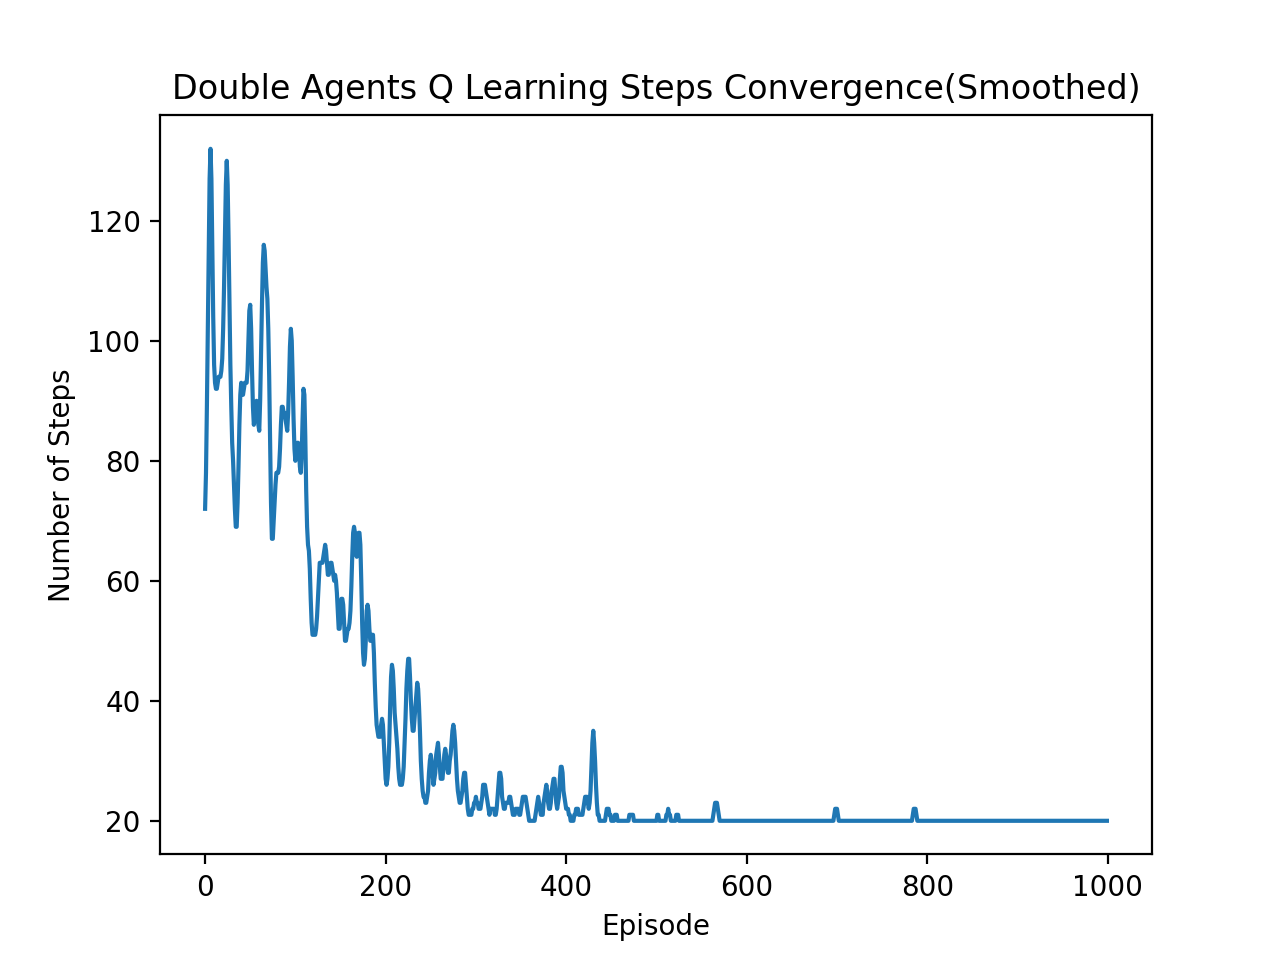
\includegraphics[width=.9\linewidth]{16.png}
     \caption{The second convergence for tabular Q learning in 4x5 gridworld}\label{Fig:Data2}
   \end{minipage}
\end{figure}

However, the number of steps that our tabular $Q$ learning generated for two drones are larger than 30 steps, the ideal minimum steps of the coverage. This means that due to the less consideration of the competitive of two drones, two drones will not visit the grids that they have already visited respectively but will repeat visiting some grids that have already been visited by another drone, showing in the figure 13, where red colored grids are grids that are visited by both agents.

\begin{figure}[H]
    \centering
    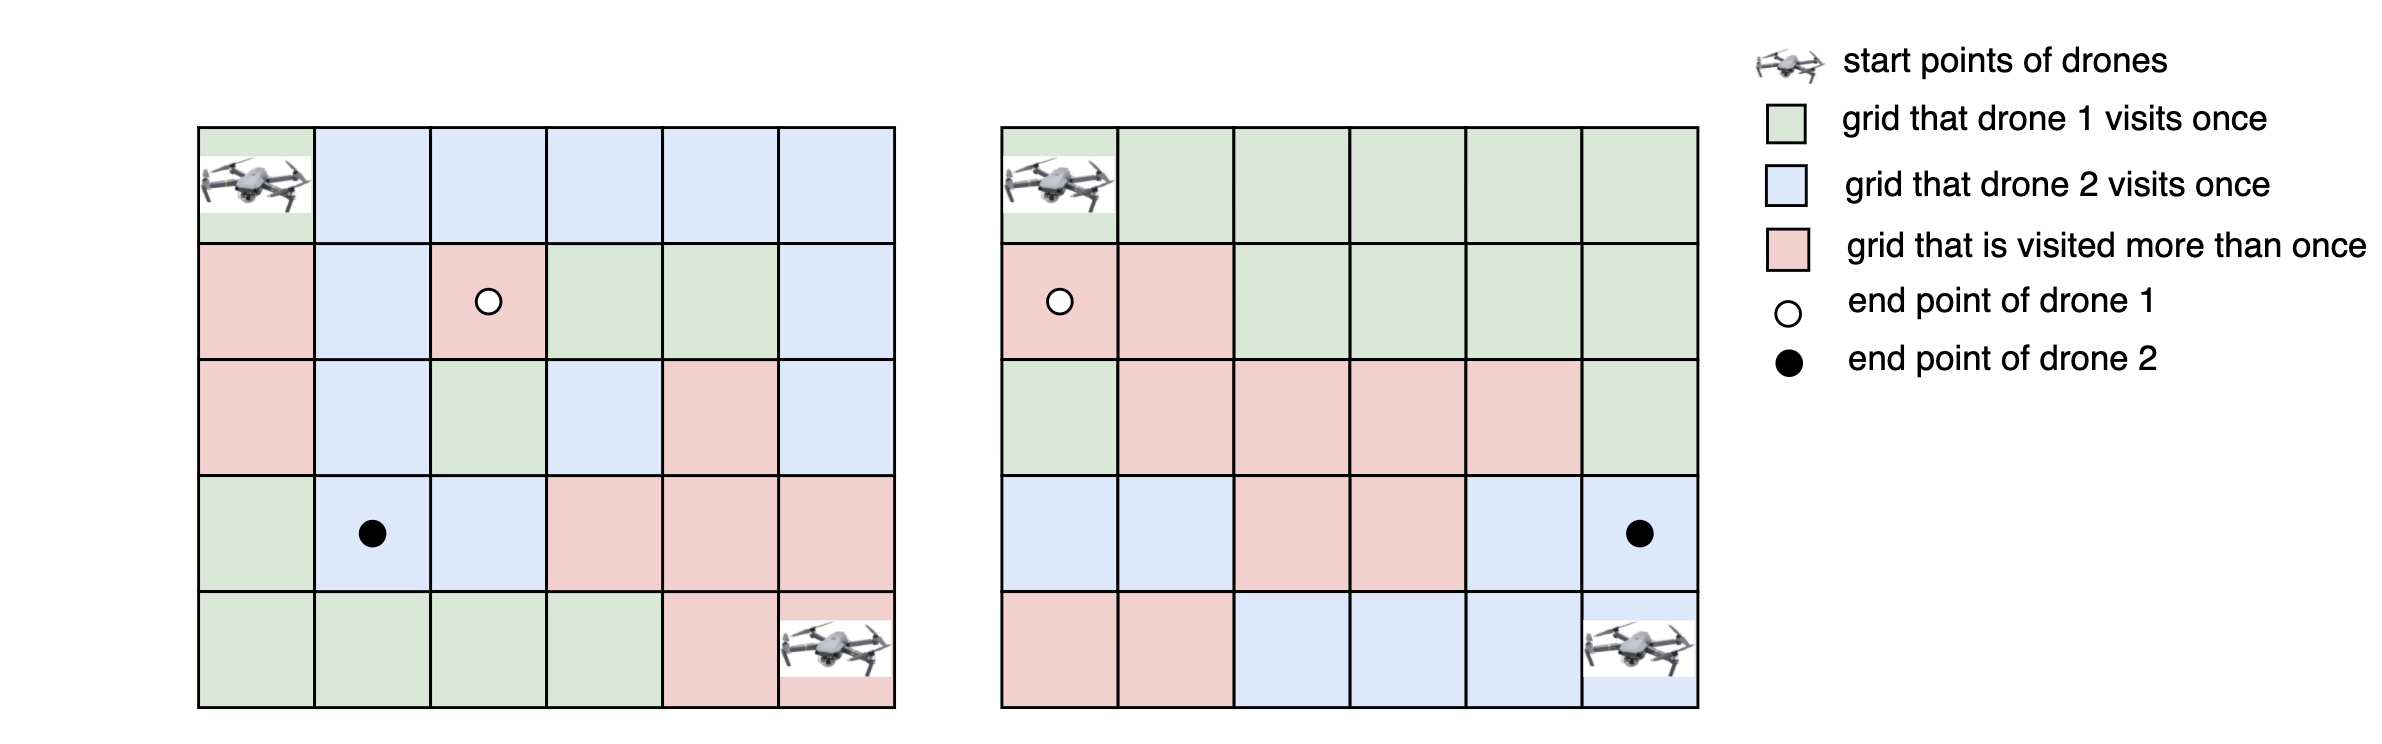
\includegraphics[width=.85\linewidth]{17.png}
    \caption{Two solutions for the double drones coverage in 5x6 gridworld}
\end{figure}
Similar with the singe agent area coverage, dual UAVs area coverage generated by our reinforcement learning method will also have different solutions for different training due to policies, and therefore end states and the number of grids that are visited for both drones are always different for our double drones tabular $Q$ learning method. As our reinforcement learning algorithm will only find the relatively short distance but not the optimal shortest distance for the coverage, and the computation for our learning will be extremely large while increasing the size of the environment, we try to find the deep reinforcement learning(DRL) method to reach our goal for the double drones area coverage. 

\subsection{Actor Critic using Kronecker-Factored Trust Region(ACKTR)}

\hspace{\parindent}As the multi-agents coverage, double agents shown in this work, requires very large state space, action space, and $Q$ table for tabular $Q$ learning, we implement the policy gradient method, actor critic using Kronecker-Factored Trust Region(ACKTR) method, to realize more stable and accurate results for double agents coverage in the gridworld. ACKTR extends the structure of natural policy gradient which performs gradient updates efficiently for both actor and critic, in comparison with normal first-order gradient method. ACKTR method also adopts the trust region formulation of the Kronecker-factored approximated curvature(K-FAC) to optimize the actor and critic\cite{ACKTR}. 

To begin with, the policy gradient method parameterize the policy $\pi_\theta(a_t|s_t)$ and update the parameter $\theta$ to maximize the objective(reward) function $J(\theta)$, defined by:

\begin{equation}
    J(\theta)=\mathbb{E}_{\pi}\left[\sum_{t=0}^{\infty} \Psi_{t} \log \pi_{\theta}\left(a_{t}|s_{t}\right)\right],
\end{equation}
where $\Psi_{t}$ is approximated as the advantage function $A^\pi$ for actor critic reinforcement learning methods, defined following the asynchronous advantage actor critic(A3C) as the $k$-step returns with function approximation\cite{A3C}, 

\begin{equation}
    A_{\theta_v}^{\pi}\left(s_{t}, a_{t}\right)=\sum_{i=0}^{k-1}\left(\gamma^{i} r\left(s_{t+i}, a_{t+i}\right)+\gamma^{k} V_{\theta_v}^{\pi}\left(s_{t+k}\right)\right)-V_{\theta_v}^{\pi}\left(s_{t}\right),
\end{equation}
where $\theta_v$ are parameters of the value network, which provides an estimate of the expected sum of rewards from the given state with policy $\pi$ \cite{rl_sutton}. 

As A3C or other deep reinforcement learning methods are usually trained by inefficient first-order stochastic gradient descent methods, ACKTR implement the natural gradient decent. The following parameters updates follow the paper \textit{Scalable trust-region method for deep reinforcement learning using Kronecker-factored approximation}\cite{ACKTR}. In ACKTR, K-FAC uses a Kronecker-factored approximation to the Fisher matrix to perform efficient approximate natural gradient updates. The Fisher metric for reinforcement learning objectives defined by policy distribution for the actor is:

\begin{equation}
    F=\mathbb{E}_{p(\tau)}\left[\nabla_\theta \log \pi\left(a_{t} | s_{t}\right) \nabla_\theta \log \pi\left(a_{t} | s_{t}\right)^{T}\right]
\end{equation}
where $\theta$ indicates weights of neural network for policy, multi-layer perceptron (MLP) network in our implementation in the Stable Baselines particularly, and
$p(\tau)$ is the distribution of trajectories given by:
\begin{equation}
    p(\tau)=p\left(s_{0}\right) \prod_{t=0}^{T} \pi\left(a_{t} | s_{t}\right) p\left(s_{t+1} | s_{t}, a_{t}\right)
\end{equation}

As in ACKTR the output of the critic $v$ is defined to be a Gaussian distribution as $p(a, v | s)=\pi(a | s) p(v | s) $, and when actor and critic share lower-layer representations, ACKTR applies K-FAC to approximate the Fisher matrix to perform updates simultaneously.

\begin{equation}
F=\mathbb{E}_{p(\tau)}\left[\nabla_\theta \log p(a, v | s) \nabla_\theta \log p(a, v | s)^{T}\right]
\end{equation}

Then, ACKTR applies trust region formulation of K-FAC, with the following updates of effective step size $\eta$ for the natural gradient:
\begin{subequations}
    \begin{align}
        \eta=\min (\eta_{\max }, & \sqrt{\frac{2 \delta}{\Delta \theta^{\mathrm{T}} \hat{F} \Delta \theta}}) \\
         \theta \leftarrow \theta-\eta & F^{-1} \nabla_{\theta} L
    \end{align}
\end{subequations}
where $\eta_{\max }$ is the learning rate and $\delta$ is the trust region radius. ACKTR is the first scalable trust region natural gradient method for actor-critic DRL, and improves the sample efficiency of current methods significantly\cite{ACKTR}. We will use this method to train our agents for the double agents coverage in the gridworld. 
We conduct our experiment for double UAVs coverage in a $10\times10$ gridworld, where the start positions for drones are the upper left and bottom right of the board respectively, and the end points are undecided to make sure that the training process is MDP. We successfully find solutions for double agents area coverage using ACKTR(\href{https://github.com/zcczhang/UAV_Coverage/tree/master/ACTKR_double_Coverage}{code}). Figure 14 shows two solutions for the coverage path planning after training 200,000 time-steps, using ACKTR implemented in the Stable Baselines in Python(\href{https://github.com/zcczhang/UAV_Coverage/tree/master/Simulation}{simulation code}).

\begin{figure}[H]
    \centering
    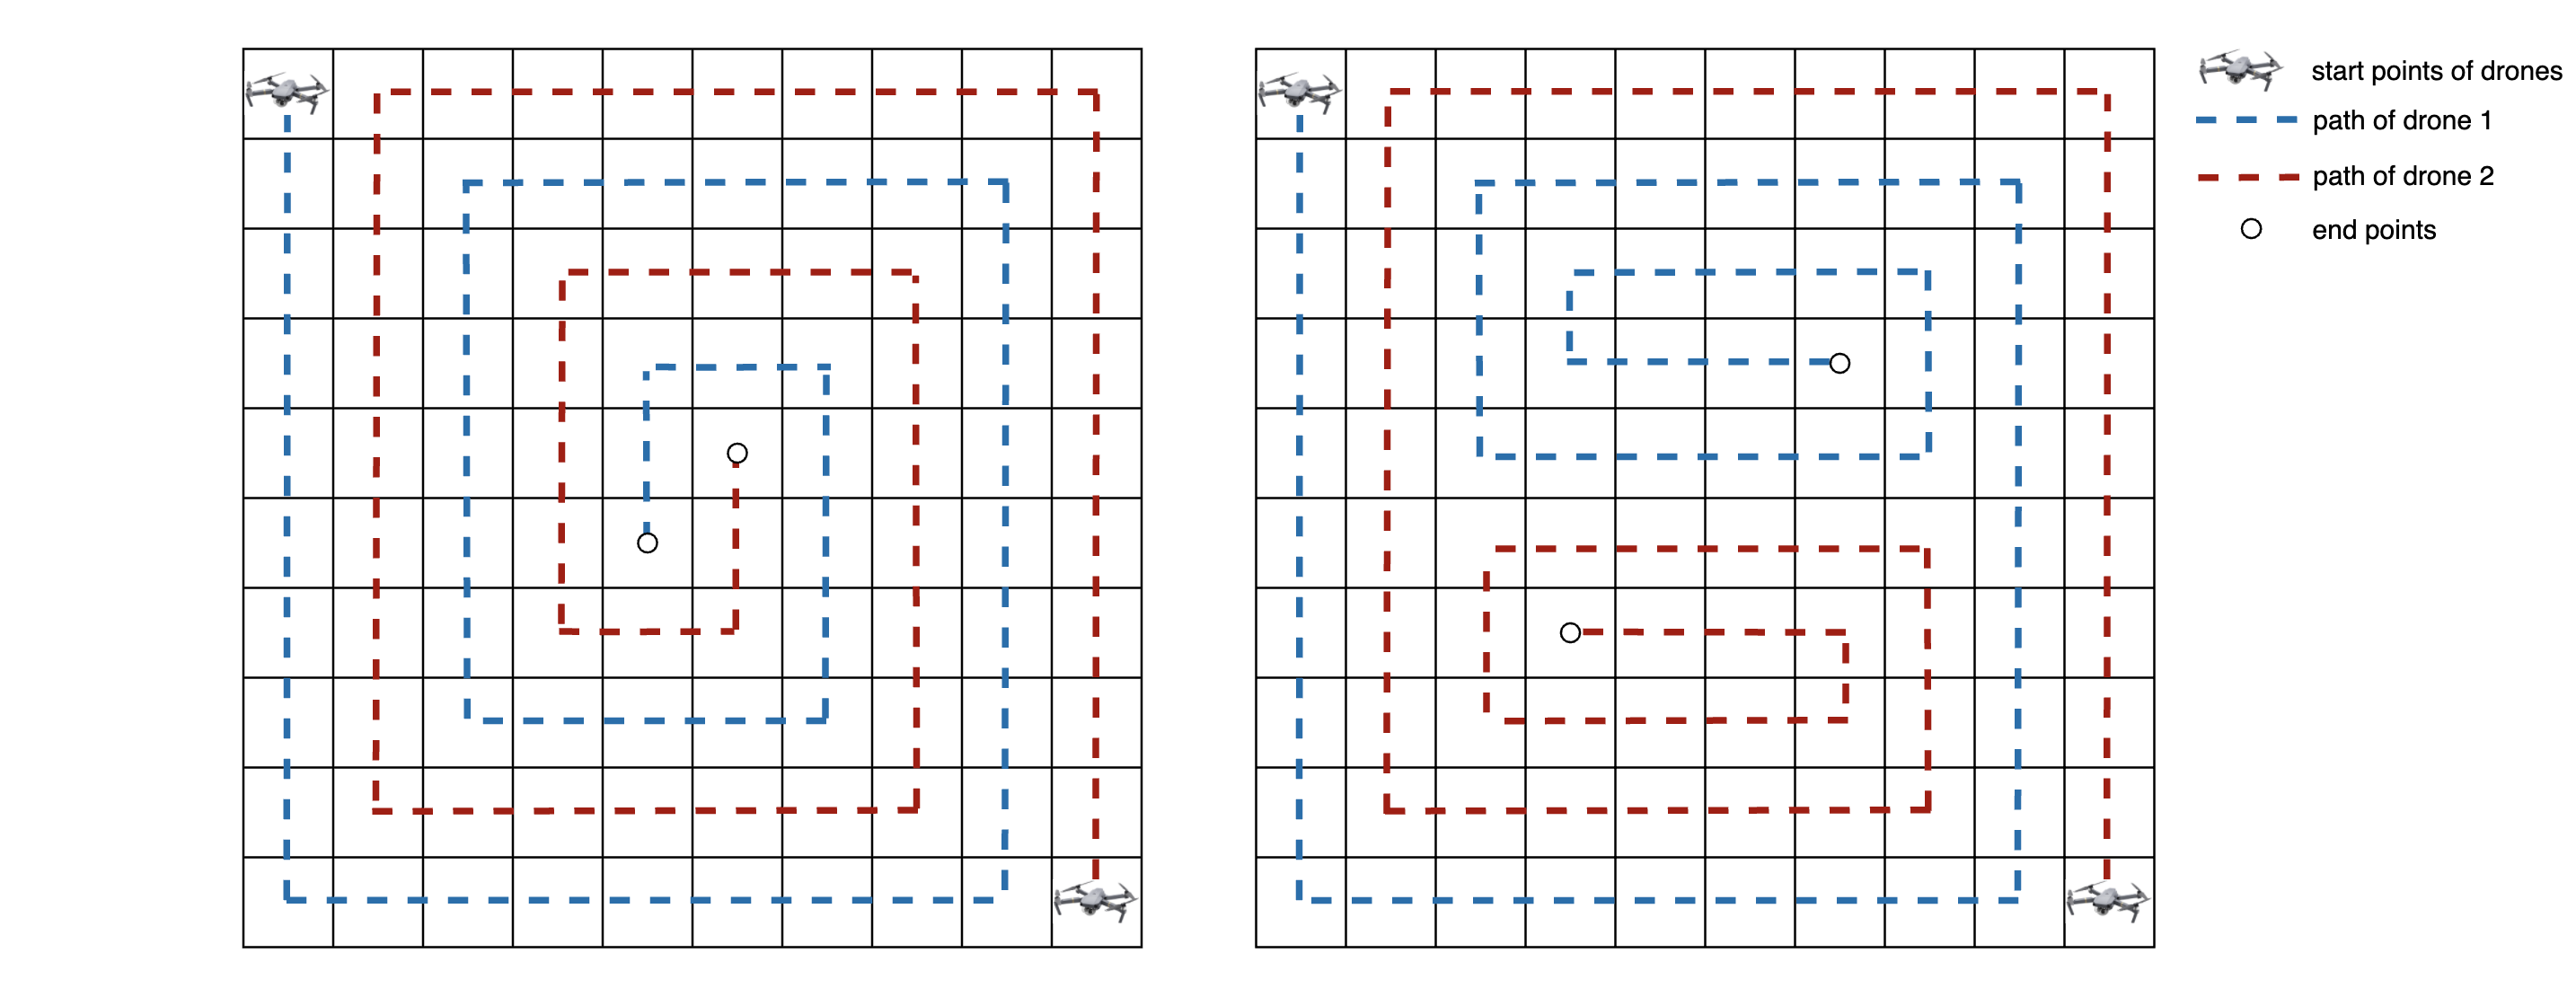
\includegraphics[width=\textwidth]{12.png}
    \caption{solutions for double agents coverage path planning in 10x10 gridworld}
\end{figure}

Figure 15 and 16 below represent the learning curve indicating the rewards the agent received each episode. The rewards received each episode are increasing overall and become stable around 70 after 150,000 time-steps. The reward feeding are typically follows Eq.\ref{eq:mrl_r}, and figure 15 and 16 illustrate how ACKTR method maximize the rewards by updating parameters of layers each time-step while training. Two figures below are learning curves indicating rewards for solutions illustrated in figure 14. The rewards are showing increasing overall and becoming stable after around 150,000 time-steps. Therefore, we could conclude that it is realizable to use ACKTR deep reinforcement learning method to complete the area coverage path planning for two agents.

\begin{figure}[H]
   \begin{minipage}{0.49\textwidth}
     \centering
     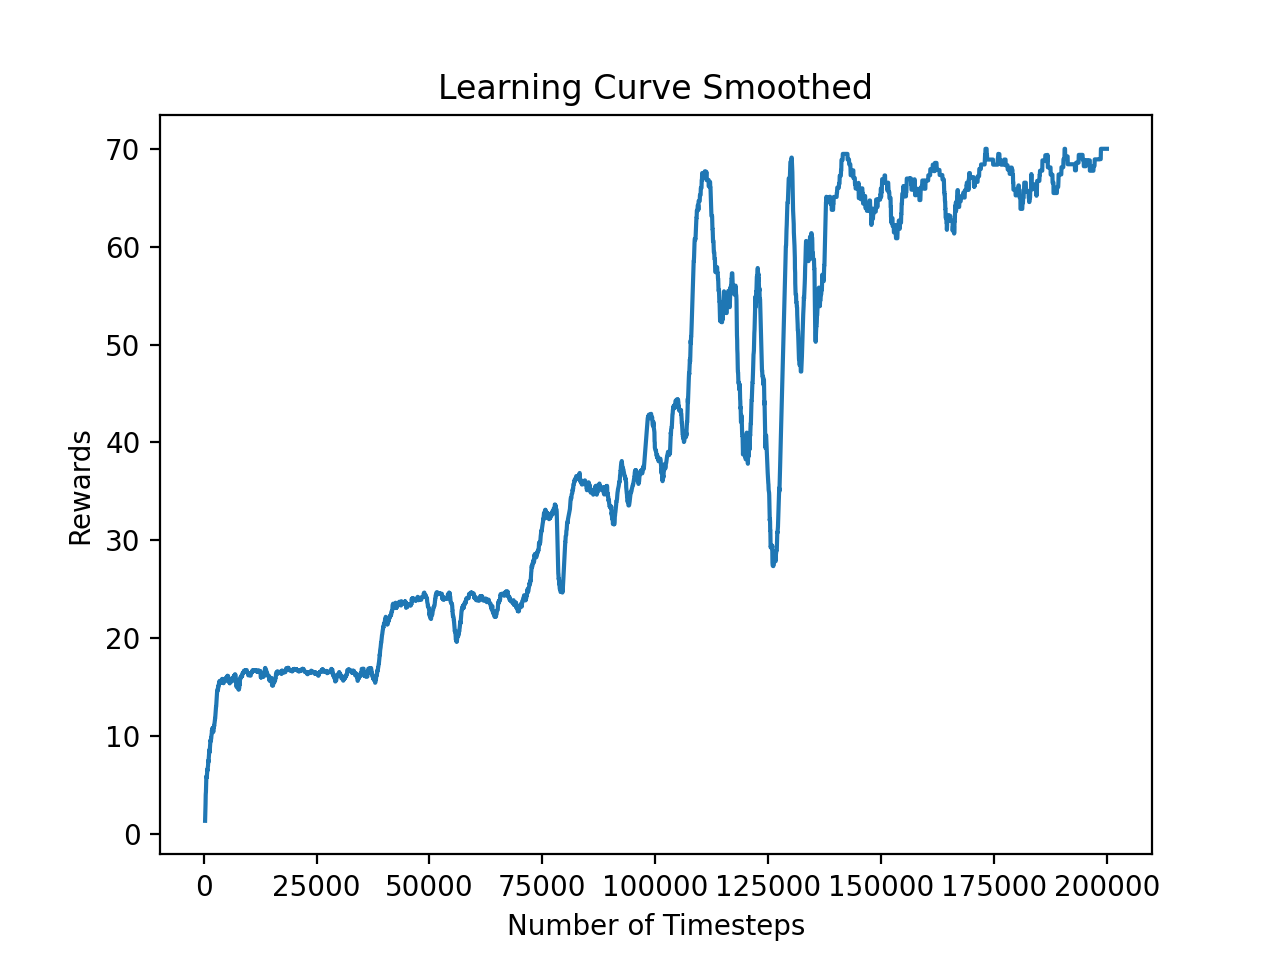
\includegraphics[width=\linewidth]{13.png}
     \caption{The first learning curve for 2 agents coverage using ACKTR in 10x10 gridworld}\label{Fig:Data1}
   \end{minipage}\hfill
   \begin{minipage}{0.49\textwidth}
     \centering
     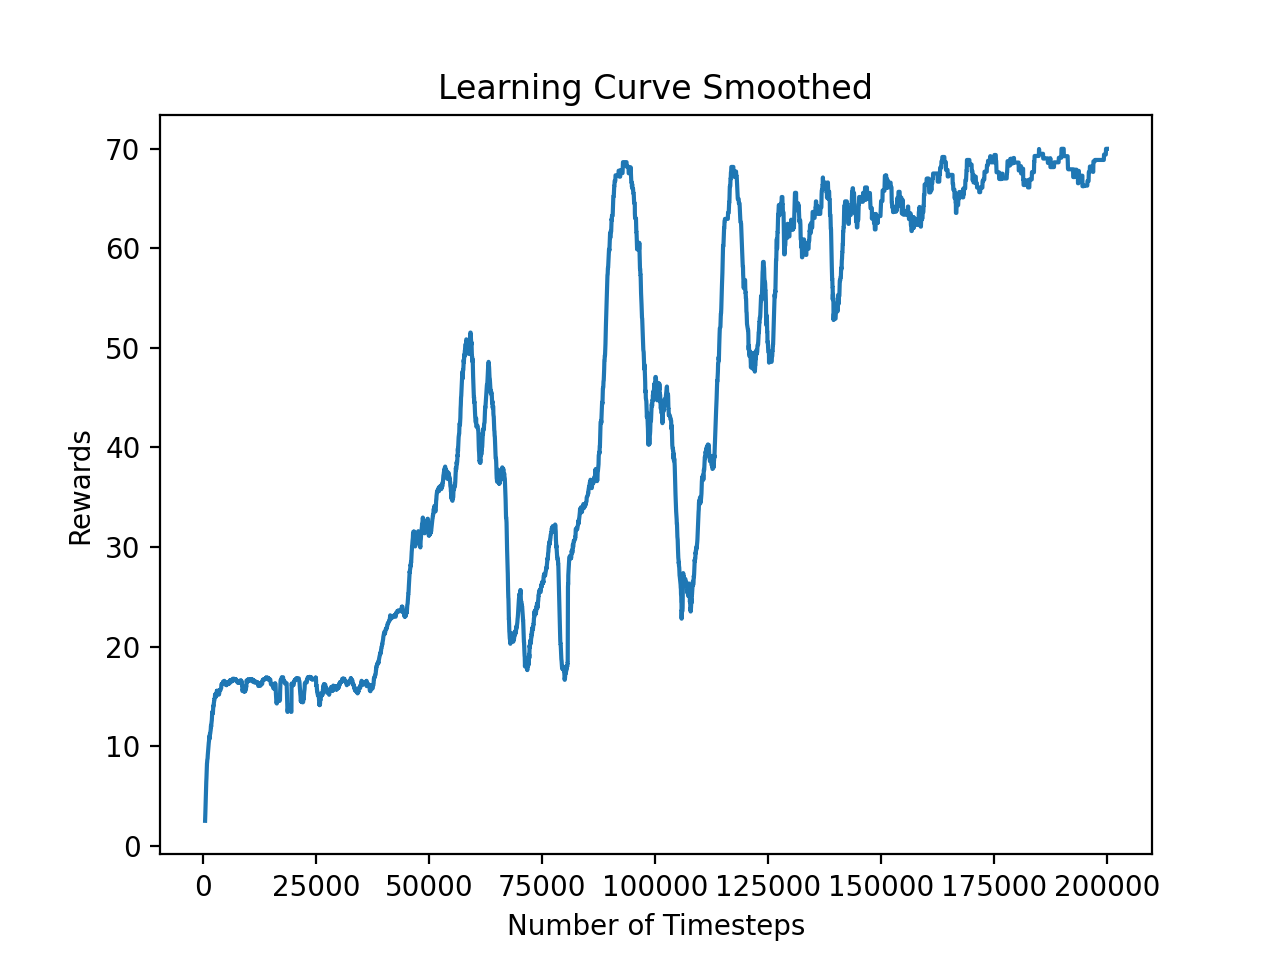
\includegraphics[width=\linewidth]{14.png}
     \caption{The second learning curve for 2 agents coverage using ACKTR in 10x10 gridworld}\label{Fig:Data2}
   \end{minipage}
\end{figure}



\section{Conclusion and Future Work}
\hspace{\parindent}In this summer research, we designed and implement efficient NMDP and MDP tabular Q learning for single drone coverage in a given regular or irregular environment, built in Gym or by graph; and ACKTR deep reinforcement learning for the double agents cooperatively learning to provide full coverage in the gridworld by Stable Baselines. The experimental results show that our reinforcement learning agents successfully learn to complete the coverage for both single and double agents, and come back to the launch position for the single agent. In the future, we are interested in using more Deep Learning methods to increase the size of the environment that can be covered with a more stable convergence, and extend it to the multi-agent systems. And we will consider energy, resolution, e.t.c. constraints in the UAV coverage in solving real life problem, such as wildfire monitoring, search and rescue missions, and so forth. It is also worth considering to apply our reinforcement learning based methods for the similar problems like Hamiltonian circuit or travelling salesman problem(TSP).

\addcontentsline{toc}{section}{Acknowledgement}
\section*{Acknowledgement}
\hspace{\parindent} This research project is funded by MacKnight-Haan-Ludwig Summer Research Collaboration Fund, Class of 1950 Summer Research Collaboration Fund, Anderson-Grossheusch Summer Research Collaboration Fund, and Mac/Faculty Collaboration Summer Research Funds. The author would like to appreciate the insightful discussion and work with Macalester College professor Esra Kadioglu-Urtis, and students Aaron Gould, Elisabeth Landgren, and Fan Zhang. 


\newpage
 \addcontentsline{toc}{section}{References}
\bibliographystyle{ieeetr}
\bibliography{reference}

\end{document}